\documentclass[a4paper]{article}

\usepackage[english]{babel}
\usepackage[utf8]{inputenc}
\usepackage{amsmath}
\usepackage{graphicx}
\usepackage[colorinlistoftodos]{todonotes}

\title{Run \#1}

%\author{Your names and group number}

\date{\today}

\begin{document}
\maketitle

\begin{abstract}
This is an attempt to try and describe how modeling the delta function as a continuous function. Right now I'm considering an extremely simple situation, where I just have a flat region with a single delta function. I approximate this delta function as a triangle, and I'm trying to figure out how the width of this triangle affects its accuracy.
\end{abstract}


\section{Generating phonon distributions}
I generated the pretend phonon distributions using the ``generateInput.py'' code. This created a series of 5 fake frequency distributions, shown below. These distributions are generated between 0 and 1, with a spacing of 0.01. The delta function is to be located at 0.5, and the area of the delta function is to be held at 0.2, while the area of the continuous piece (the flat piece) is to be held at 1.0. 

\begin{figure}
\centering
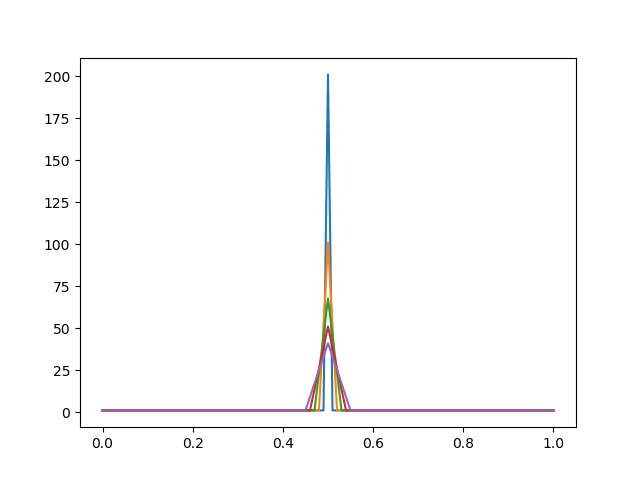
\includegraphics[width=1.0\textwidth]{phononDist_run1}
\caption{\label{fig:run1}Fake frequency distributions of run 1. For this I consider five different continuous representations of a delta function, each a triangle with varying width. }
\end{figure}





%\section{Intro}
%\label{sec:introduction}
%\cite{nano3}.

%\section{Theory 2-3 pages}
%\label{sec:theory}

%\subsection{Two-dimensional Electron Gas}

%\subsection{Quantum Hall Effect}

%\begin{figure}
%\centering
%\includegraphics[width=1\textwidth]{raw_data.png}
%\caption{\label{fig:data}Raw (unprocessed) data. Replace this figure with the one you've made, that shows the resistivity.}
%\end{figure}
%

%\newpage
%\begin{figure}
%\centering
%\includegraphics[width=0.3\textwidth]{frog.jpg}
%\caption{\label{fig:frog}this frog was uploaded to writelatex via the project menu.}
%\end{figure}


%\begin{table}
%\centering
%\begin{tabular}{l|r}
%Item & Quantity \\\hline
%Widgets & 42 \\
%Gadgets & 13
%\end{tabular}
%\caption{\label{tab:widgets}An example table.}
%\end{table}

%\begin{equation}
%S_n = \frac{X_1 + X_2 + \cdots + X_n}{n}
%      = \frac{1}{n}\sum_{i}^{n} X_i
%\label{eq:sn}
%\end{equation}
%
%denote their mean. Then as $n$ approaches infinity, the random variables $\sqrt{n}(S_n - \mu)$ converge in distribution to a normal $\mathcal{N}(0, \sigma^2)$.

%The equation \ref{eq:sn} is very nice.


%\subsection{How to Make Lists}

%You can make lists with automatic numbering \dots

%\begin{enumerate}
%\item Like this,
%\item and like this.
%\end{enumerate}
%\dots or bullet points \dots
%\begin{itemize}
%\item Like this,
%\item and like this.
%\end{itemize}
%\dots or with words and descriptions \dots
%\begin{description}
%\item[Word] Definition
%\item[Concept] Explanation
%\item[Idea] Text
%\end{description}


%\begin{thebibliography}{9}
%\bibitem{nano3}
%  K. Grove-Rasmussen og Jesper Nygård,
%  \emph{Kvantefænomener i Nanosystemer}.
%  Niels Bohr Institute \& Nano-Science Center, Københavns Universitet
%
%\end{thebibliography}


\end{document}
